\documentclass[11pt,]{article}
\usepackage[left=1in,top=1in,right=1in,bottom=1in]{geometry}
\newcommand*{\authorfont}{\fontfamily{phv}\selectfont}
\usepackage[]{mathpazo}


  \usepackage[T1]{fontenc}
  \usepackage[utf8]{inputenc}



\usepackage{abstract}
\renewcommand{\abstractname}{}    % clear the title
\renewcommand{\absnamepos}{empty} % originally center

\renewenvironment{abstract}
 {{%
    \setlength{\leftmargin}{0mm}
    \setlength{\rightmargin}{\leftmargin}%
  }%
  \relax}
 {\endlist}

\makeatletter
\def\@maketitle{%
  \newpage
%  \null
%  \vskip 2em%
%  \begin{center}%
  \let \footnote \thanks
    {\fontsize{18}{20}\selectfont\raggedright  \setlength{\parindent}{0pt} \@title \par}%
}
%\fi
\makeatother




\setcounter{secnumdepth}{0}


\usepackage{graphicx}
% We will generate all images so they have a width \maxwidth. This means
% that they will get their normal width if they fit onto the page, but
% are scaled down if they would overflow the margins.
\makeatletter
\def\maxwidth{\ifdim\Gin@nat@width>\linewidth\linewidth
\else\Gin@nat@width\fi}
\makeatother
\let\Oldincludegraphics\includegraphics
\renewcommand{\includegraphics}[1]{\Oldincludegraphics[width=\maxwidth]{#1}}

\title{Global Effects Of The Mexico City Policy  }



\author{\Large Joshua Keating, Peter Freschi, and John Harrison\vspace{0.05in} \newline\normalsize\emph{University of Washington}  }


\date{}

\usepackage{titlesec}

\titleformat*{\section}{\normalsize\bfseries}
\titleformat*{\subsection}{\normalsize\itshape}
\titleformat*{\subsubsection}{\normalsize\itshape}
\titleformat*{\paragraph}{\normalsize\itshape}
\titleformat*{\subparagraph}{\normalsize\itshape}


\usepackage{natbib}
\bibliographystyle{apsr}



\newtheorem{hypothesis}{Hypothesis}
\usepackage{setspace}

\makeatletter
\@ifpackageloaded{hyperref}{}{%
\ifxetex
  \usepackage[setpagesize=false, % page size defined by xetex
              unicode=false, % unicode breaks when used with xetex
              xetex]{hyperref}
\else
  \usepackage[unicode=true]{hyperref}
\fi
}
\@ifpackageloaded{color}{
    \PassOptionsToPackage{usenames,dvipsnames}{color}
}{%
    \usepackage[usenames,dvipsnames]{color}
}
\makeatother
\hypersetup{breaklinks=true,
            bookmarks=true,
            pdfauthor={Joshua Keating, Peter Freschi, and John Harrison (University of Washington)},
             pdfkeywords = {Mexico City policy, Global Gag Rule},  
            pdftitle={Global Effects Of The Mexico City Policy},
            colorlinks=true,
            citecolor=blue,
            urlcolor=blue,
            linkcolor=magenta,
            pdfborder={0 0 0}}
\urlstyle{same}  % don't use monospace font for urls



\begin{document}
	
% \pagenumbering{arabic}% resets `page` counter to 1 
%
% \maketitle

{% \usefont{T1}{pnc}{m}{n}
\setlength{\parindent}{0pt}
\thispagestyle{plain}
{\fontsize{18}{20}\selectfont\raggedright 
\maketitle  % title \par  

}

{
   \vskip 13.5pt\relax \normalsize\fontsize{11}{12} 
\textbf{\authorfont Joshua Keating, Peter Freschi, and John Harrison} \hskip 15pt \emph{\small University of Washington}   

}

}







\begin{abstract}

    \hbox{\vrule height .2pt width 39.14pc}

    \vskip 8.5pt % \small 

\noindent This document provides an introduction to R Markdown, argues for its
benefits, and presents a sample manuscript template intended for an
academic audience. I include basic syntax to R Markdown and a minimal
working example of how the analysis itself can be conducted within R
with the \texttt{knitr} package.


\vskip 8.5pt \noindent \emph{Keywords}: Mexico City policy, Global Gag Rule \par

    \hbox{\vrule height .2pt width 39.14pc}



\end{abstract}


\vskip 6.5pt

\noindent  \section{Introduction}\label{introduction}

The issue of abortion in the United States is one that is fiercely
debated and divides large segments of the population. These divides are
inherently partisan and therefore have led to legislation. In 1984 the
Reagan administration signed into law the ``Mexico City policy'', named
for the city in which it was signed. The policy requires all non
governmental organizations operating abroad to refrain from performing,
advising on or endorsing abortion as a method of family planning if they
wish to continue to receive receive federal funding. The policy has had
a tumultuous history, either being reinstated or rescinded depending on
the party affiliation of the current president. Starting with Bill
Clinton in 1993 the policy was rescinded, then restored by George W.
Bush in 2001, rescinded again by Barack Obama in 2009, and most recently
restored by Donald J. Trump in 2017.

At it's heart, the ban is propelled by the desire to limit the use of
U.S. taxpayer dollars to pay for abortion or abortion-related services.
The consequences of this ban include the termination of abortion related
services such as; education, family planning, counseling, and training.
The all or nothing nature of the ban would also cut off funds for non
abortion related health services that would be offered at non
governmental health providers. This presents some serious public health
concerns for areas of the world where these services are essential for
maternal health and prenatal care.

We hypothesized that the institution of the ban could lead to a
reduction in family planning services which could then lead to an
increase in induced abortions. By restricting the flow of funds into
health clinics that provide services related to abortion among others,
the U.S. government restricts the amount of care that can be provided to
those utilizing those services. The aim of this project was to gather,
analyze, and present data on the past effects of the Global Gag Rule and
create a resource that assists our audience in understanding the scope
of the policy, its observable impact on women's health, and the pathways
through which it influences public health policy decisions outside of
the United States.

\section{Related Work}\label{related-work}

The United Nations' Department of Economic and Social Affairs has
conducted various research via nationally-representative surveys. Their
dataset\footnote{World Contraceptive Use 2016, includes country-specific
  estimates of these and other indicators, based on survey data
  available as of April 2016
  \href{http://www.un.org/en/development/desa/population/publications/dataset/contraception/wcu2016.shtml}{dataset
  link}} (World Contraceptive Use 2016) contains information about
prevalence and unmet family planning needs for 195 different
countries/areas of the world from 1950 to 2015. This information is
broken down by type of contraceptive and specific demand for family
planning through different methods, which was gathered through about 15
conducted surveys across the world. These types of indicators are
effective in assessing the progress of universal reproductive
health-care and family planning information in a geographical area. The
global gag rule has been known to threaten the funding of certain
health-care organizations, which may have effects on the prevalence of
contraceptive and family planning methods.

The World Health Organization (WHO) published a study\footnote{United
  States aid policy and induced abortion in sub-Saharan Africa
  \href{http://www.who.int/bulletin/volumes/89/12/11-091660/en/}{study},
  \href{http://www.who.int/bulletin/volumes/89/12/BLT-11-091660-table-T1.html}{dataset}}
in partnership with the Stanford University Department of Medicine in
2011 analysing the effects of the ``Mexico City Policy'' on a set of
sub-Saharan African countries. Specifically, this study attempted to
determine whether a relationship exists between the reinstatement of the
Mexico City Policy and the probability that a sub-Saharan African woman
will have an induced abortion. The Stanford researchers looked at the
relationship between a country's exposure to the Mexico City Policy and
the odds of abortion among women of reproductive age between 1994 and
2008. In this way they were able to find a statistically
significant\footnote{Women living in highly exposed countries had 2.73
  (95\% CI: 1.95--3.82) times the odds of having an induced abortion
  after the policy's reinstatement than during the period from 1994 to
  2000 or than women living in less exposed countries.
  \href{http://www.who.int/bulletin/volumes/89/12/BLT-11-091660-table-T3.html}{summary}}
relationship between the introduction of the Mexico City Policy and an
increase in induced abortions.

The U.S. Administration of International Development, as the major
government agency in international aid, is responsible for reporting all
official U.S. foreign aid to Congress. USAID maintains an extensively
detailed database for reporting this data, which keeps records of
foreign aid obligations and disbursements back to 1946. In addition to
storing and reporting this data, USAID provides many projects under
Barack Obama's open government initiative in order to encourage public
collaboration on research and data analysis. The Foreign Aid
Explorer\footnote{USAID is responsible for reporting official U.S.
  Government foreign aid to Congress and the Organization for Economic
  Cooperation and Development (OECD)
  \href{https://explorer.usaid.gov/aid-dashboard.html}{Foreign Aid
  Explorer website}} provides a dashboard for querying and downloading
this dataset, but also includes its own visualizations and maps that
provide informative breakdowns of global financial aid. This project was
invaluable for obtaining and becoming familiar with the USAID dataset we
performed analysis on.

\section{Methods}\label{methods}

While the World Contraceptive Use 2016 dataset included levels of
contraceptive and family planning methods for an extensive number of
countries across the world, we chose to analyze a certain subset of this
data. After the raw excel data was downloaded from the United Nations'
website, it required a substantial amount of cleaning because of the
format of the column headers. Once the columns were renamed, records for
countries in Sub-Saharan Africa were aggregated over time using dplyr.
Reproductive health metrics for married/in-union women of reproductive
age were examined across the time periods where the Mexico City Policy
was active and inactive in the United States.

In approaching this analysis we needed to use some unconventional
methods of data sourcing. For the data on induced abortions and exposure
to the ``Global Gag Rule'' (GGR) we scraped a \texttt{.html} table that
the WHO made available through the Stanford paper published on their
website. Unfortunately for me, the hierarchy of the table did not easily
lend itself to reshaping in R so a considerable amount of work was done
to convert it into a long form \texttt{.csv} file. We were curious about
some of the potential public health effects that the ban could have had
historically on an area such as maternal mortality. The hypothesis that
maternal mortality would be higher after the ban was instituted was
based on our intuition. We used a dataset from the World Health
Organization covering maternal mortality rates from 1990 to 2015 for
every country. From there we broke the data into subsets to focus on the
20 sub-Saharan countries that we had exposure data on and added those
rates onto our dataset. After we had a complete dataset we performed a
linear regression to gauge whether our hypothesis was correct. In the
model we used the variation in policy exposure compared against
variation in the rates of maternal mortality while subsetting for
abortion rates in the targeted countries.

(PUT JOHNS METHODS HERE)

\section{Results}\label{results}

At vero eos et accusamus et iusto odio dignissimos ducimus qui
blanditiis praesentium voluptatum deleniti atque corrupti quos dolores
et quas molestias excepturi sint occaecati cupiditate non provident,
similique sunt in culpa qui officia deserunt mollitia animi, id est
laborum et dolorum fuga. Et harum quidem rerum facilis est et expedita
distinctio. Nam libero tempore, cum soluta nobis est eligendi optio
cumque nihil impedit quo minus id quod maxime placeat facere possimus,
omnis voluptas assumenda est, omnis dolor repellendus. Temporibus autem
quibusdam et aut officiis debitis aut rerum necessitatibus saepe eveniet
ut et voluptates repudiandae sint et molestiae non recusandae. Itaque
earum rerum hic tenetur a sapiente delectus, ut aut reiciendis
voluptatibus maiores alias consequatur aut perferendis doloribus
asperiores repellat

\section{Discussion}\label{discussion}

At vero eos et accusamus et iusto odio dignissimos ducimus qui
blanditiis praesentium voluptatum deleniti atque corrupti quos dolores
et quas molestias excepturi sint occaecati cupiditate non provident,
similique sunt in culpa qui officia deserunt mollitia animi, id est
laborum et dolorum fuga. Et harum quidem rerum facilis est et expedita
distinctio. Nam libero tempore, cum soluta nobis est eligendi optio
cumque nihil impedit quo minus id quod maxime placeat facere possimus,
omnis voluptas assumenda est, omnis dolor repellendus. Temporibus autem
quibusdam et aut officiis debitis aut rerum necessitatibus saepe eveniet
ut et voluptates repudiandae sint et molestiae non recusandae. Itaque
earum rerum hic tenetur a sapiente delectus, ut aut reiciendis
voluptatibus maiores alias consequatur aut perferendis doloribus
asperiores repellat

\begin{figure}
\centering
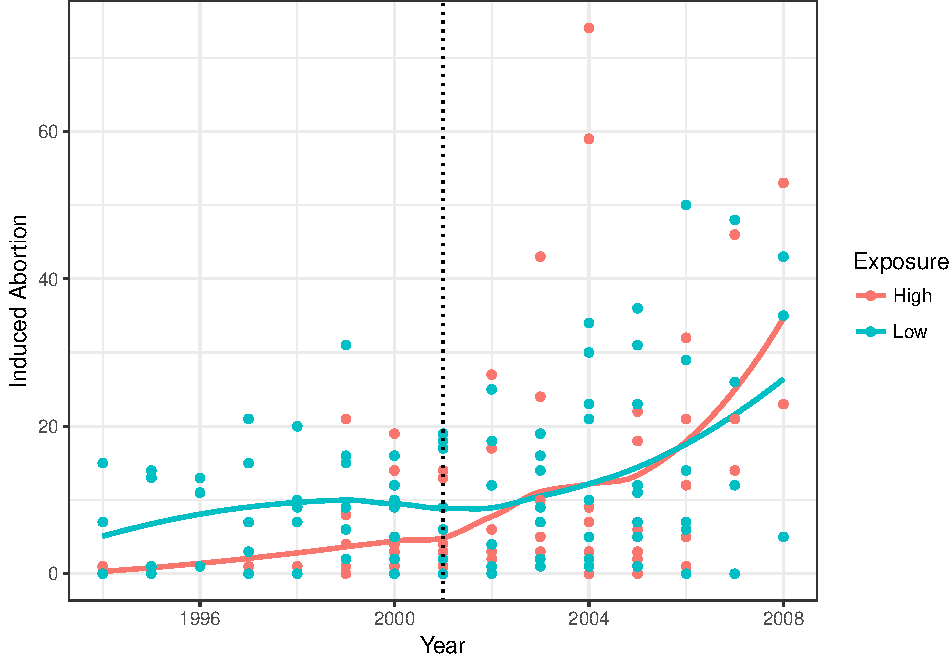
\includegraphics{final-paper_files/figure-latex/unnamed-chunk-1-1.pdf}
\caption{Test}
\end{figure}

\section{Future Work}\label{future-work}

At vero eos et accusamus et iusto odio dignissimos ducimus qui
blanditiis praesentium voluptatum deleniti atque corrupti quos dolores
et quas molestias excepturi sint occaecati cupiditate non provident,
similique sunt in culpa qui officia deserunt mollitia animi, id est
laborum et dolorum fuga. Et harum quidem rerum facilis est et expedita
distinctio. Nam libero tempore, cum soluta nobis est eligendi optio
cumque nihil impedit quo minus id quod maxime placeat facere possimus,
omnis voluptas assumenda est, omnis dolor repellendus. Temporibus autem
quibusdam et aut officiis debitis aut rerum necessitatibus saepe eveniet
ut et voluptates repudiandae sint et molestiae non recusandae. Itaque
earum rerum hic tenetur a sapiente delectus, ut aut reiciendis
voluptatibus maiores alias consequatur aut perferendis doloribus
asperiores repellat

\newpage
\singlespacing 
\end{document}
